\documentclass{article}

\usepackage{fancyhdr}
\usepackage{extramarks}
\usepackage{amsmath}
\usepackage{amsthm}
\usepackage{amsfonts}
\usepackage{tikz}
\usepackage[plain]{algorithm}
\usepackage{algpseudocode}
\usepackage{graphicx}
\graphicspath{{./images/}{IR}}

\usetikzlibrary{automata,positioning}

%
% Basic Document Settings
%

\topmargin=-0.45in
\evensidemargin=0in
\oddsidemargin=0in
\textwidth=6.5in
\textheight=9.0in
\headsep=0.25in

\linespread{1.1}

\pagestyle{fancy}
\lhead{\hmwkAuthorName}
\chead{\hmwkClass\ (\hmwkClassInstructor\ \hmwkClassTime): \hmwkTitle}
\rhead{\firstxmark}
\lfoot{\lastxmark}
\cfoot{\thepage}

\renewcommand\headrulewidth{0.4pt}
\renewcommand\footrulewidth{0.4pt}

\setlength\parindent{0pt}

%
% Create Problem Sections
%

\newcommand{\enterProblemHeader}[1]{
    \nobreak\extramarks{}{Problem \arabic{#1} continued on next page\ldots}\nobreak{}
    \nobreak\extramarks{Problem \arabic{#1} (continued)}{Problem \arabic{#1} continued on next page\ldots}\nobreak{}
}

\newcommand{\exitProblemHeader}[1]{
    \nobreak\extramarks{Problem \arabic{#1} (continued)}{Problem \arabic{#1} continued on next page\ldots}\nobreak{}
    \stepcounter{#1}
    \nobreak\extramarks{Problem \arabic{#1}}{}\nobreak{}
}

\setcounter{secnumdepth}{0}
\newcounter{partCounter}
\newcounter{homeworkProblemCounter}
\setcounter{homeworkProblemCounter}{1}
\nobreak\extramarks{Problem \arabic{homeworkProblemCounter}}{}\nobreak{}

%
% Homework Problem Environment
%
% This environment takes an optional argument. When given, it will adjust the
% problem counter. This is useful for when the problems given for your
% assignment aren't sequential. See the last 3 problems of this template for an
% example.
%
\newenvironment{homeworkProblem}[1][-1]{
    \ifnum#1>0
        \setcounter{homeworkProblemCounter}{#1}
    \fi
    \section{Problem \arabic{homeworkProblemCounter}}
    \setcounter{partCounter}{1}
    \enterProblemHeader{homeworkProblemCounter}
}{
    \exitProblemHeader{homeworkProblemCounter}
}

%
% Homework Details
%   - Title
%   - Due date
%   - Class
%   - Section/Time
%   - Instructor
%   - Author
%

\newcommand{\hmwkTitle}{Homework\ \#1}
\newcommand{\hmwkDueDate}{October 25, 2020}
\newcommand{\hmwkClass}{CS445/545}
\newcommand{\hmwkClassTime}{}
\newcommand{\hmwkClassInstructor}{Dr. A. Rhodes}
\newcommand{\hmwkAuthorName}{\textbf{Austen Nelson}}

%
% Title Page
%

\title{
    \vspace{2in}
    \textmd{\textbf{\hmwkClass:\ \hmwkTitle}}\\
    \normalsize\vspace{0.1in}\small{Due\ on\ \hmwkDueDate\ at 3:10pm}\\
    \vspace{0.1in}\large{\textit{\hmwkClassInstructor\ \hmwkClassTime}}
    \vspace{3in}
}

\author{\hmwkAuthorName}
\date{}

\renewcommand{\part}[1]{\textbf{\large Part \Alph{partCounter}}\stepcounter{partCounter}\\}

%
% Various Helper Commands
%

% Useful for algorithms
\newcommand{\alg}[1]{\textsc{\bfseries \footnotesize #1}}

% For derivatives
\newcommand{\deriv}[1]{\frac{\mathrm{d}}{\mathrm{d}x} (#1)}

% For partial derivatives
\newcommand{\pderiv}[2]{\frac{\partial}{\partial #1} (#2)}

% Integral dx
\newcommand{\dx}{\mathrm{d}x}

% Alias for the Solution section header
\newcommand{\solution}{\textbf{\large Solution}}

% Probability commands: Expectation, Variance, Covariance, Bias
\newcommand{\E}{\mathrm{E}}
\newcommand{\Var}{\mathrm{Var}}
\newcommand{\Cov}{\mathrm{Cov}}
\newcommand{\Bias}{\mathrm{Bias}}

\begin{document}

\maketitle

\pagebreak

\begin{homeworkProblem}
   \textbf{Experiment 1: Vary number of hidden units}

   This scatter plot shows how changing the number of neurons in the hidden layer
   affected the rate of training of the network. The dotted lines represent the training
   set and the solid lines are the corresponding test sets. Values of 20, 50, and 100 were 
   chosen for the dimension of the hidden layer. The learning rate was fixed to 0.1, momentum
   to 0.9, and weights were initialized to random values between -0.05 and 0.05. The networks
   were trained for 50 epochs and the accuracy as well as a confusion matrix was recorded at
   the end of each epoch on both a disjoint test set and the training set. The confusion matrices
   shown are from epoch 10, as the networks didn't improve after that point.

   \begin{figure}[h!]
      \centering
      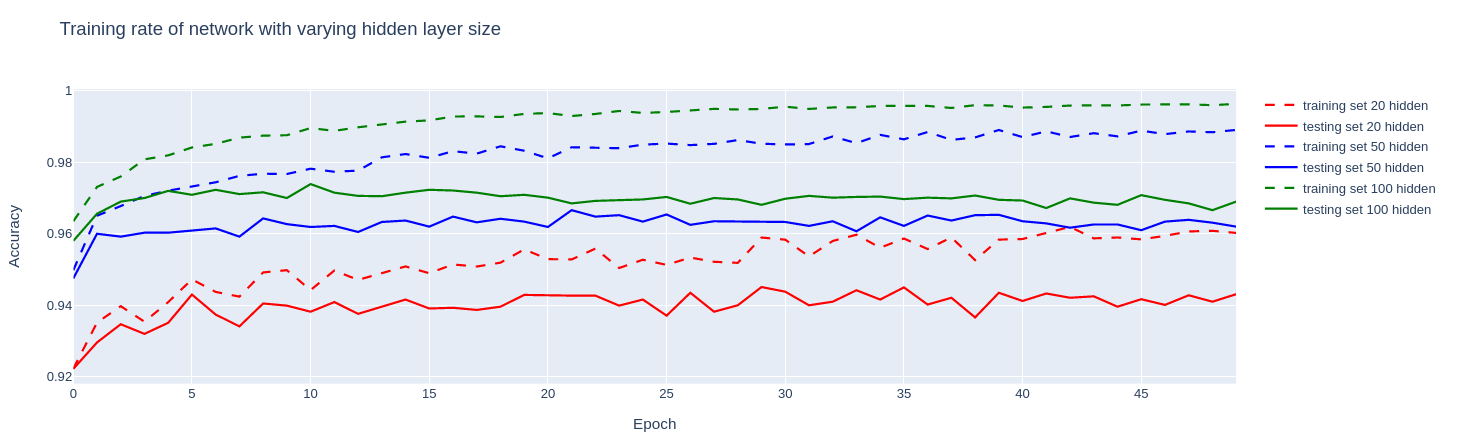
\includegraphics[width=0.8\linewidth]{hidden_scatter.png}
      \caption[fig1]{hidden scatter}
   \end{figure}

   \begin{figure}[h!]
      \centering
      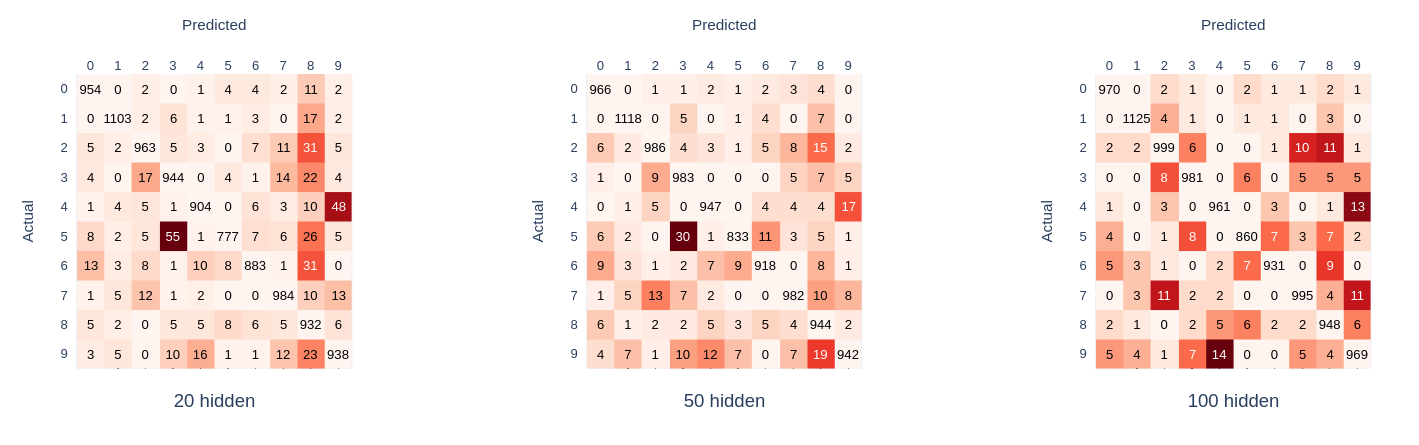
\includegraphics[width=0.8\linewidth]{hidden_confusion.png}
      \caption[fig2]{hidden confusion}
   \end{figure}

   \textbf{1. How does the number of hidden units affect the final accuracy on the test data?}
   For the three levels of hidden units I tested, increasing the number of hidden units correlated
   with an increase in overall accuracy of the network. This is expected because it allows for
   more complex neural pathways to emerge during training. Looking at the confusion matrices,
   the 20 and 50 unit networks had a difficult time identifying 5's by mistaking them as 3's.
   The 100 unit network seems to have figured this difference out but at the cost of minor
   loss of accuracy of other numbers. It is also interesting to note that 20 and 50 would mistake
   5's as 3's but rarely 3's as 5's, where the 100 unit network had similar accuracy between these
   pairs. 

   \textbf{2. How does it affect the number of epochs needed for training to converge?}
   It seems that increasing the number of hidden units slightly increased the amount of training
   needed to converge the network. 20 hit near its best on the 5th epoch, 50 on the 8th, and 100
   on the 10th. 20 and 50 both had accuracies that barely exceeded these early maximums in later
   epochs but after significant oscillation in accuracy. This leads me to believe that these later
   peaks aren't meaningful. The oscillation in accuracy after the initial maximums decreases as
   number of hidden neurons increased, but none of the networks really benefited from more that
   10 epochs of training on the test set.

   \textbf{3. Is there evidence that any of your networks has overfit to the training data?
   If so, what is that evidence?}
   There is evidence that all 3 of the networks were overfit. Each network did not improve much
   after 10 epochs on the test set, and the 20 got worse. For all the networks the accuracy on
   the training set gradually increased well beyond the 10th epoch demonstrating some level of 
   memorization happening.

   \textbf{4. How do your results compare to the results obtained by your perceptron in HW 1?}
   Which homework?

\end{homeworkProblem}

\begin{homeworkProblem}
   \textbf{Experiment 2: Vary the momentum value}

   This scatter plot shows how changing the momentum value affected the rate of training of the
   network. Values of 0, 0.25, 0.5, and 0.9 were chosen for the momentum coefficient for each
   network. Hidden units was fixed at 100, the learning rate at 0.1, and weights were initialized
   to values between -0.05 and 0.05. The confusion matrices were taken from the 10th epoch.

   \begin{figure}[h!]
      \centering
      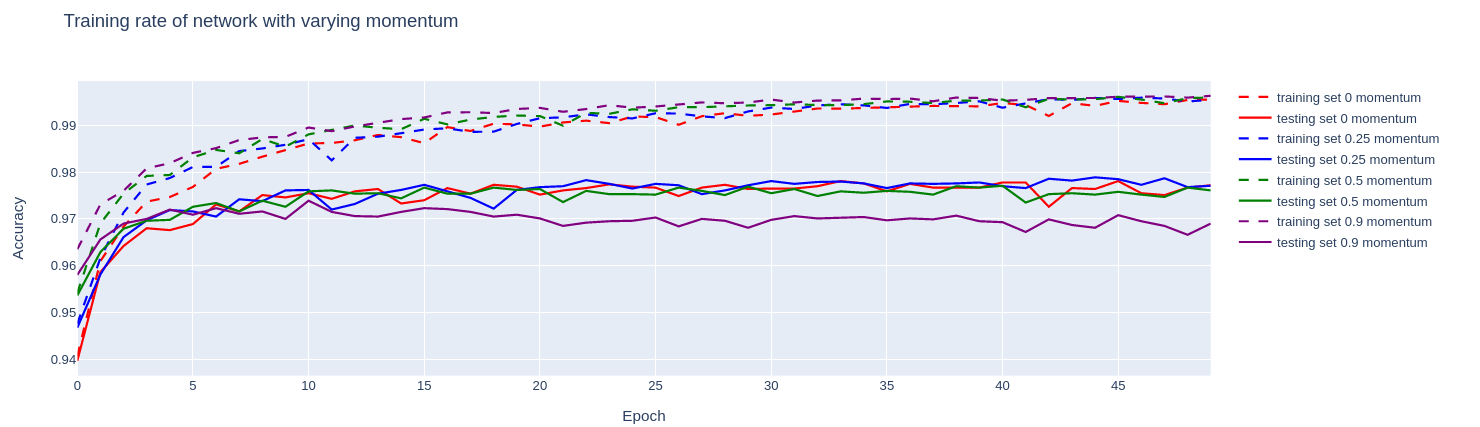
\includegraphics[width=0.8\linewidth]{momentum_scatter.png}
      \caption[fig1]{momentum scatter}
   \end{figure}

   \begin{figure}[h!]
      \centering
      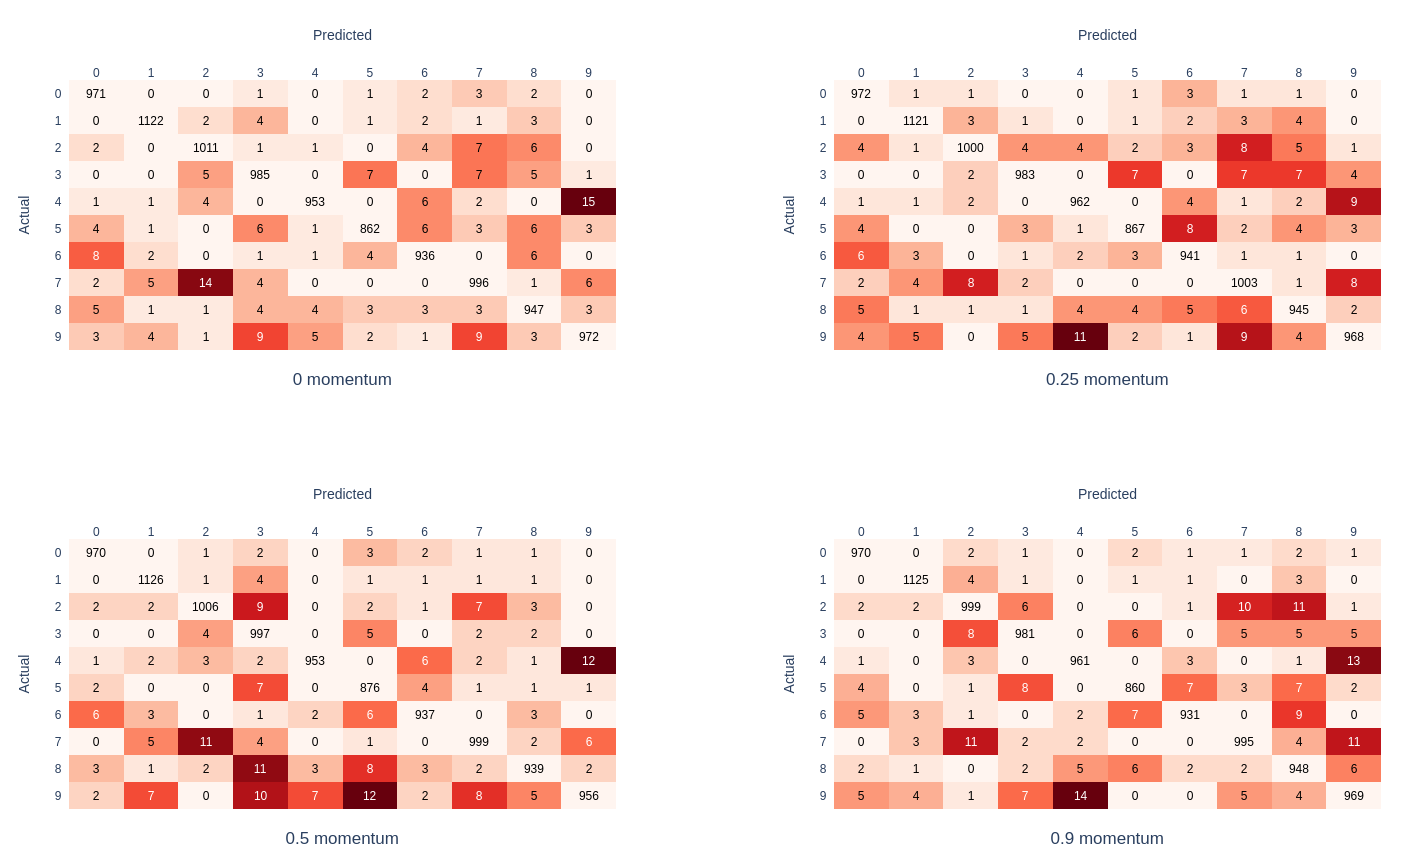
\includegraphics[width=0.8\linewidth]{momentum_confusion.png}
      \caption[fig2]{momentum confusion}
   \end{figure}

   \textbf{How does the momentum value affect the final accuracy on the test data?}
   The momentum value had little effect on the maximum accuracy of the network, but higher
   momentum was more prone to overfitting. The 0.9 momentum started to diverge from the other
   networks in accuracy around 10 epochs. This seems intuitive as a higher momentum is going
   to begin memorizing the training set faster.

   \textbf{How does it affect the number of epochs needed for training to converge?}
   For the first 3 to 5 epochs, the larger momentums approached their maximum accuracy faster.
   This is also intuitive. Between 5 and 10 epochs, though, there seems to be little difference.

   \textbf{Again, is there evidence that any of your networks has overfit to the training data?}
   Again, there is little improvement after 10 epochs. This suggests overfitting because the
   accuracy of the training set continues to improve where the accuracy of the test sets 
   oscillates or decreases. As mentioned in the first question, it seems that higher momentums
   are more prone to overfitting.

\end{homeworkProblem}

\begin{homeworkProblem}
   \textbf{Experiment 3: Vary the number of training examples}

   This scatter plot shows how changing the number of training examples affects the rate of
   training of the network. $\frac{1}{4}$ (15,000), $\frac{1}{2}$ (30,000), and all (60,000)
   of the examples were used for each network. Hidden units was fixed at 100, momentum to 0.9,
   and weights were initialized to values between -0.05 and 0.05. The confusion matrices of the
   training set were checked to make sure an even proportion of examples was used in each network.
   The confusion matrices shown are from the 10th epoch of the test set on these networks.

   \begin{figure}[h!]
      \centering
      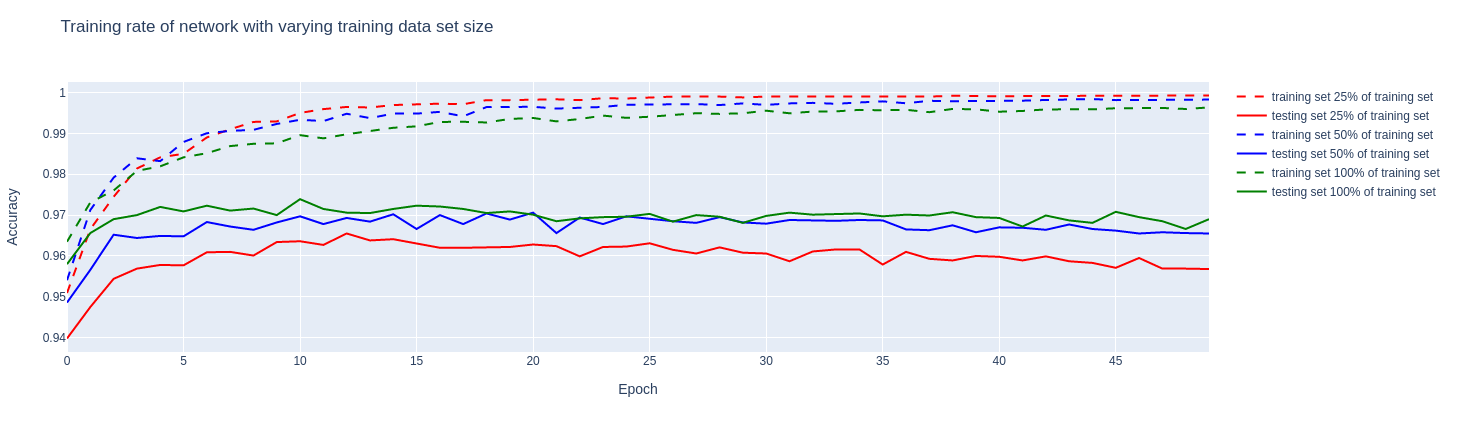
\includegraphics[width=0.8\linewidth]{test_set_size_scatter.png}
      \caption[fig1]{test set size scatter}
   \end{figure}

   \begin{figure}[h!]
      \centering
      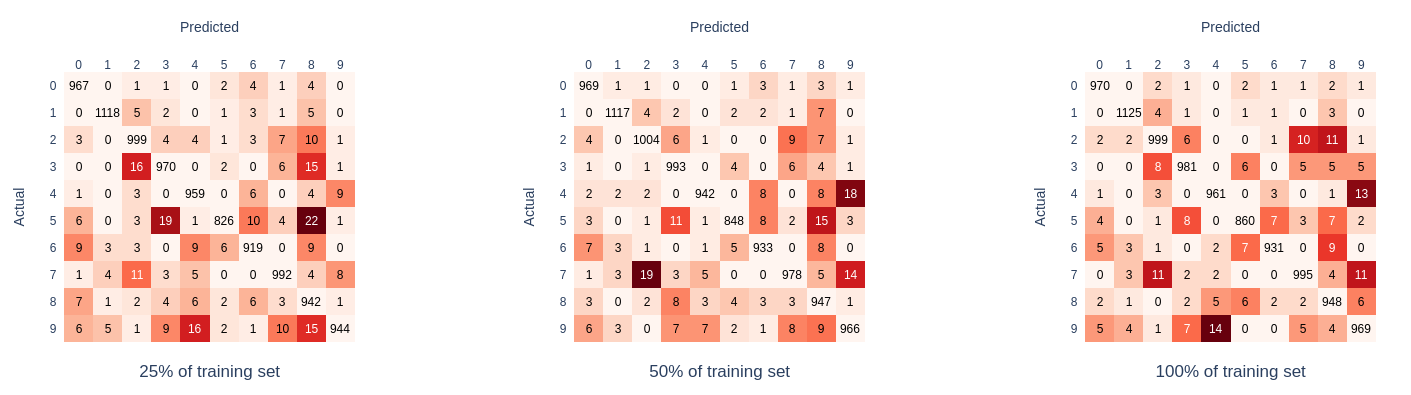
\includegraphics[width=0.8\linewidth]{test_set_size_confusion.png}
      \caption[fig2]{test set size confusion}
   \end{figure}

   \textbf{How does the size of the training data affect the final accuracy on the test data?}
   Reducing the number of training examples has a clear affect of reducing the maximum accuracy
   of the network. Although the half and full set are fairly close, there is nearly an entire
   percent difference in accuracy from the quarter network.

   \textbf{How does it affect the number of epochs needed for training to converge?}
   The networks with more training examples also converged at the maximum accuracy faster. 
   The full train set network was nearing its maximum as early as the 4th epoch, the half around
   the 6th, and the quarter peaked at 12. This is also intuitive because with more data you are
   doing more adjustment per epoch.

   \textbf{Again, is there evidence that any of your networks has overfit to the training data?}
   Again, beyond 10 all the networks started to do worse on test accuracy but training accuracy
   slowly increased. I am surprised the training accuracy for the quarter network took the longest
   to level off because there is less data to memorize but it makes sense that less training data
   is simply just less adjustment per epoch. The quarter network was significantly more
   susceptible to overtraining and really started to fall off earlier that the other two networks.
\end{homeworkProblem}

\end{document}
